\documentclass{beamer}

\usepackage{algorithm}
\usepackage{algpseudocode}
\usepackage{amsfonts,amsbsy,amsthm,amsmath,amssymb}
\usepackage{beamerthemesplit}
\usepackage{comment}
\usepackage{listings}
\usepackage{multirow}

\DeclareMathOperator*{\argmax}{arg\,max}
\DeclareMathOperator*{\argmin}{arg\,min}
\DeclareMathOperator{\ord}{ord}
\DeclareMathOperator{\sign}{sign}

\algtext*{EndWhile}      % Remove "end while" text
\algtext*{EndIf}         % Remove "end if" text
\algtext*{EndFor}        % Remove "end for" text
\algtext*{EndProcedure}  % Remove "end procedure" text
\renewcommand{\algorithmiccomment}[1]{\hfill \{#1\}}
\renewcommand{\algorithmicrequire}{\textbf{Input:}}
\renewcommand{\algorithmicensure}{\textbf{Output:}}
\newcommand{\algnewline}{\par\noindent\hskip\algorithmicindent}

\newcommand{\CC}{\mathbb{C}}
\newcommand{\NN}{\mathbb{N}}
\newcommand{\RR}{\mathbb{R}}
\newcommand{\ZZ}{\mathbb{Z}}
\newcommand{\QQ}{\mathbb{Q}}
\newcommand{\RRgtz}{\mathbb{R}_{>0}}
\newcommand{\ZZgtz}{\mathbb{Z}_{>0}}
\newcommand{\ZZgez}{\mathbb{Z}_{\ge 0}}
\newcommand{\QQgtz}{\mathbb{Q}_{>0}}
\newcommand{\QQgez}{\mathbb{Q}_{\ge 0}}

\newcommand{\KK}{\mathcal{K}}
\newcommand{\MM}{\mathcal{M}}
\newcommand{\OO}{\mathcal{O}}

\newcommand{\matrixto}[2]{\left[ \begin{array}{rr} #1 & #2 \end{array} \right]}
\newcommand{\matrixot}[2]{\left[ \begin{array}{r} #1 \\ #2 \end{array} \right]}
\newcommand{\matrixtt}[4]{\left[ \begin{array}{rr} #1 & #2 \\ #3 & #4 \end{array} \right]}
\newcommand{\matrixltt}[4]{\left[ \begin{array}{ll} #1 & #2 \\ #3 & #4 \end{array} \right]}
\newcommand{\matrixThreeOne}[3]{\left[ \begin{array}{rrr} #1 & #2 & #3 \end{array} \right]}
\newcommand{\matrixThreeTwo}[6]{\left[ \begin{array}{rrr} #1 & #2 & #3 \\ #4 & #5 & #6 \end{array} \right]}
\newcommand{\ntoinfty}{\lim_{n \rightarrow \infty}}
\newcommand{\floor}[1]{\left\lfloor #1 \right\rfloor}
\newcommand{\ceil}[1]{\left\lceil #1 \right\rceil}

\newcommand{\band}{~\texttt{and}_\texttt{2}~}
\newcommand{\bor}{~\texttt{or}_\texttt{2}~}
\newcommand{\bxor}{\oplus}
\newcommand{\bnot}{\lnot}
\newcommand{\binary}[1]{\texttt{#1}_\texttt{2}}

\newcommand{\set}{\mathcal}
\newcommand{\ideal}{\mathfrak}
\newcommand{\idealclass}[1]{\left[ \ideal #1 \right]}
\newcommand{\aclass}{\idealclass a}
\newcommand{\bclass}{\idealclass b}
\newcommand{\cclass}{\idealclass c}
\newcommand{\dclass}{\idealclass d}
\newcommand{\pclass}{\idealclass p}
\newcommand{\qclass}{\idealclass q}
\newcommand{\idclass}{[\mathcal O_\Delta]}

\newcommand{\ith}{i^{\textrm{th}}}

\newcommand{\smallfont}{\fontsize{6pt}{7.2}\selectfont}

\graphicspath{{eps/}{png/}{l2r-best-approx/}}

\title[]{SuperSPAR}
\subtitle{An Integer Factoring Algorithm}
\author{Maxwell Sayles}
\date{May 24, 2013}
\institute{
	\bigskip 
       Department of Computer Science \\
       University of Calgary
}

\usetheme{Copenhagen}
\setbeamertemplate{navigation symbols}{} %no nav symbols

\makeatletter
\setbeamertemplate{footline}
{%
  \leavevmode%
  \hbox{\begin{beamercolorbox}[wd=.5\paperwidth,ht=2.5ex,dp=1.125ex,leftskip=.3cm plus1fill,rightskip=.3cm]{author in head/foot}%
    \usebeamerfont{author in head/foot} \hspace*{2em} SuperSPAR \hspace*{2em}
  \end{beamercolorbox}%
  \begin{beamercolorbox}[wd=.5\paperwidth,ht=2.5ex,dp=1.125ex,leftskip=.3cm,rightskip=.3cm plus1fil]{title in head/foot}%
      \usebeamerfont{title in head/foot} \hspace*{2em} \insertframenumber ~/ 61 \hspace*{2em}
%    \usebeamerfont{title in head/foot} \hspace*{2em} \insertframenumber ~/ \inserttotalframenumber \hspace*{2em}
  \end{beamercolorbox}}%
  \vskip0pt%
}
\makeatother


\begin{document}
\maketitle

% OVERVIEW
\begin{frame}
\frametitle{Overview}
What is SuperSPAR?
\begin{itemize}[<+->]
\item Improves upon SPAR (named after Shanks, Pollard, Atkin, and Rickert).
\item Based on arithmetic in the ideal class group of imaginary quadratic number fields.
\item Uses the order of an element in this group to factor an integer.
\end{itemize}
\end{frame}

\begin{frame}
\frametitle{Binary Quadratic Forms}
Ideal class group originally studied by Gauss.
\begin{itemize}
\item<2-> $Q(x, y) = ax^2 + bxy + cy^2$
\item<3-> $Q(x, y) = 2x^2 + xy + 18y^2 \break
= \{2,8,18,19,21,24,28,32,33,39,46,50,54,63,72,...\}$
\item<4-> $\Delta = b^2 - 4ac$
\item<5-> $\Delta = 1^2 - 4 \cdot 2 \cdot 18 = -143$
\item<6-> Extremely rich theory.
\item<7-> Different properties when $\Delta < 0$ or $\Delta > 0$.
\end{itemize}
\end{frame}

\begin{frame}
\frametitle{Equivalence of Forms}
Two forms are equivalent
\[
Q(x, y) \sim Q'(x',y')
\]
if there exists an invertible integral linear transformation
\begin{align*}
x &= \alpha x' + \beta y' \\
y &= \gamma x' + \delta y'.
\end{align*}
\end{frame}
\begin{frame}
\frametitle{Equivalence of Forms}
Substituting and simplifying give
\begin{eqnarray*}
ax^2 + bxy + cy^2
	&=& a(\alpha x' + \beta y')^2 \\
	&& + b(\alpha x' + \beta y')(\gamma x' + \delta y') \\
	&& + c(\gamma x' + \delta y')^2 \\
	&=& a'{x'}^2 + b'x'y' + c'{y'}^2
\end{eqnarray*}
\end{frame}

% EQUIVALENCE EXAMPLE
\begin{frame}
\frametitle{Example of Equivalent Forms}
\[
92x^2-26xy+6y^2 ~ \sim ~ 6{x'}^2+2x'y'+64{y'}^2
\]
is given by the transformation
\[
\matrixtt{\alpha}{\beta}{\gamma}{\delta} = \matrixtt{2}{1}{1}{0}
\]
\end{frame}

% EQUIVALENCE CLASS
\begin{frame}
\frametitle{Equivalence Class of Binary Quadratic Forms}
An \emph{equivalence class} is the set of all forms equivalent to a given form.

\bigbreak
Similar to modular arithmetic:
\begin{align*}
0 &\equiv 7, 14, 21, 28, 35, 42, ... \pmod 7 \\
1 &\equiv 8, 15, 22, 29, 36, 43, ... \pmod 7 \\
2 &\equiv 9, 16, 23, 30, 37, 44, ... \pmod 7 \\
3 &\equiv 10, 17, 24, 31, 38, 45, ... \pmod 7 \\
4 &\equiv 11, 18, 25, 32, 39, 46, ... \pmod 7 \\
5 &\equiv 12, 19, 26, 33, 40, 47, ... \pmod 7 \\
6 &\equiv 13, 20, 27, 34, 41, 48, ... \pmod 7
\end{align*}
\end{frame}

% REDUCED FORMS
\begin{frame}
\frametitle{Reduced Forms}
Work in reduced forms:
\[
-a < b \le a < c \textrm{ or } 0 \le b \le a = c.
\]

\bigbreak
Bounds:
\[
-\Delta = 4ac - b^2 \ge 4ac-a^2 \ge 3a^2
\]
gives
\[
|b| \le a \le \sqrt{|\Delta|/3} \textrm{ and } c \le |\Delta|/4.
\]

\bigbreak
\smallfont
${}^*$ Only holds for $\Delta < 0$.
\end{frame}

% IDEAL REDUCTION
\begin{frame}
\frametitle{Ideal Reduction}
\begin{algorithmic}[1]
\Require $(a, b, c)$ and $\Delta$.
\While {$a > c$ or $b > a$ or $b \le -a$}
	\If {$a > c$}
		\State swap $a$ with $c$ and set $b \gets -b$
	\EndIf
	\If {$b > a$ or $b \le -a$}
		\State $b \gets b'$ such that $-a < b' \le a$ and $b' \equiv b \pmod{2a}$
		\State $c \gets (b^2-\Delta)/4a$
	\EndIf
\EndWhile
\If {$a=c$ and $b < 0$}
	\State $b \gets -b$
\EndIf
\State \Return $(a, b, c)$
\end{algorithmic}
\end{frame}

% REDUCTION EXAMPLE
\begin{frame}
\frametitle{REDUCTION EXAMPLE}
\begin{align*}
Q(x, y) &= 72x^2 + 130xy + 64y^2 \\
&\sim 64x^2 -130xy + 72y^2 \\
&\sim 64x^2 -2xy + 6y^2 \\
&\sim 6x^2 +2xy +64y^2
\end{align*}
\end{frame}

% CONCEPTUAL MULTIPLICATION
\begin{frame}
\frametitle{Multiplication of Forms}
\begin{align*}
Q_1(x, y) &= 2x^2 + xy + 18y^2 \\
&= \{2,8,18,19,21,24,28,32,33,39,46,50,54,63,72,...\} \\
Q_2(x, y) &= 3x^2 +xy +12y^2 \\
&= \{3,12,14,16,22,26,27,36,42,48,49,53,56,64,69,...\} \\
\\
R(x,y) &= Q_1(x,y) \cdot Q_2(x,y) \\
&= 6x^2 + xy + 6y^2 \\
&= \{6,24,28,32,44,52,54,57,63,72,84,96,98,99,112...\}
\end{align*}
\end{frame}


% IDEAL MULTIPLICATION
\begin{frame}
\frametitle{Ideal Multiplication}
\begin{algorithmic}[1]
\Require Ideals $(a_1, b_1, c_1)$, $(a_2, b_2, c_2)$, and $\Delta$.
\State $s = \gcd(a_1, a_2, (b_1+b_2)/2) = Ya_1 + Va_2 + W(b_1+b_2)/2$
\State $U = (V(b_1-b_2)/2 - Wc_2) \bmod{(a_1/s)}$
\State $a = (a_1a_2)/s^2$
\State $b = (b_2 + 2Ua_2/s) \bmod{2a}$
\State $c = (b^2 - \Delta)/4a$
\end{algorithmic}
\end{frame}

% IDEAL MULTIPLICATION
\begin{frame}
\frametitle{Split XGCD}

Split $s = \gcd(a_1, a_2, (b_1+b_2)/2) = Ya_1 + Va_2 + W(b_1+b_2)/2$ into two computations.
\bigbreak

\begin{algorithmic}[1]
\Require Ideals $(a_1, b_1, c_1)$, $(a_2, b_2, c_2)$, and $\Delta$.
\State $s' = \gcd(a_1, a_2) = Y'a_1 + V'a_2$ \Comment{$Y'$ is never used}
\If {$s' = 1$}
\State $s = 1, V = V', W = 0$
\Else
\State $s = \gcd(s', (b_1 + b_2)/2) = V''s' + W(b_1 + b_2)/2$
\State $V = V'V''$ 
\EndIf
\State ...
\end{algorithmic}
\end{frame}

% NUCOMP
\begin{frame}
\frametitle{Simultaneous Multiplication and Reduction}
NUCOMP -- due to Shanks with improvements by Jacobson, Williams, Imbert, and Schmidt.
\begin{itemize}[<+->]
\item $a_1, a_2 \le \sqrt{|\Delta|/3}$, but the product $a \le |\Delta|/3$.
\item Reduction is the simple continued fraction expansion of $b/2a$.
\item $b/2a \approx sU/a_1$.
\item Derive the reduced product from the simple continued fraction expansion.
\item Simplifies when squaring and cubing.
\end{itemize}
\end{frame}

% IDENTITY
\begin{frame}
\frametitle{Identity}
Denoted $1_G$:
\[
(a, b, c) = \begin{cases}
  (1, 0, \Delta/4) & \textrm{when } \Delta \equiv 0 \pmod 4 \\
  (1, 1, (1-\Delta)/4) & \textrm{when } \Delta \equiv 1 \pmod 4
\end{cases}
\]
\end{frame}

% INVERSE
\begin{frame}
\frametitle{Inverse}
\[
(a, b, c)^{-1} = (a, -b, c)
\]
\end{frame}

% CLASS GROUP
\begin{frame}
\frametitle{Class Group of Binary Quadratic Forms}
Class group is 
\begin{itemize}
\item closed,
\item associative,
\item commutative,
\item has identity,
\item has inverse
\end{itemize}
 -- finite Abelian group.
\end{frame}

% AMBIGUOUS FORM
\begin{frame}
\frametitle{How Does this Factor an Integer?}
Ambiguous form is any form $q$ such that $q^2 = 1_G$.

\bigbreak
Three varieties:
\begin{align*}
(a, 0, c) &\Rightarrow \Delta = -4ac \\
(a, a, c) &\Rightarrow \Delta = a^2 - 4ac = a(a - 4c) \\
(a, b, a) &\Rightarrow \Delta = b^2 - 4a^2 = (b+2a)(b-2a)
\end{align*}

Choose some form with $\Delta = -kN$.
\end{frame}

% FINDING AN AMBIGUOUS FORM
\begin{frame}
\frametitle{Finding an Ambiguous Form}
Let $h = \ord(q)$ such that $q^h = 1_G$.

\bigbreak
If $h$ is even, then let $h'$ be the odd part of $h$ and
\[
	{q^{h'}}^{\left(2^j\right)}
\]
is an ambiguous form.
\end{frame}

% FINDING THE ORDER
\begin{frame}
\frametitle{How Do We Find the Order?}
\begin{itemize}
\item Exponentiate $q^E$ for $E = \prod {p_i}^{e_i}$ for odd primes $p_i$.
\item Use an order finding algorithm. 
\end{itemize}
\end{frame}



%%%%%%%%%%%%%%%%%%%%%%%%%%%%%%%%%%%%%%%%%%%%%%%%%%%%%%%%%%%%%%%%%%%%%%%%%%%%%%%%
  
% IMPROVE IDEAL ARITHMETIC
\begin{frame}
\frametitle{Improvements to Group Arithmetic}
\begin{itemize}
\item Implementations for 64-bit and 128-bit arithmetic.
\item Full/Partial extended greatest common divisor.
	\begin{itemize}
	\item Implementations of XGCD for 32-bit, 64-bit, 128-bit arithmetic.
	\end{itemize}
\end{itemize}
\end{frame}

% XGCD
\begin{frame}
\frametitle{How to Compute XGCD?}
Start with
\begin{align*}
s &= Ua + Vb \\
t &= Xa + Yb
\end{align*}
with
\[
\matrixThreeTwo{s}{U}{V}{t}{X}{Y} \gets \matrixThreeTwo{a}{1}{0}{b}{0}{1}.
\]
Maintain $s \ge t \ge 0$.
\end{frame}

% EEA
\begin{frame}
\frametitle{Extended Euclidean Algorithm}
\begin{algorithmic}[1]
\Procedure{EEA}{$a, b$} \Comment{$a, b \in \ZZgez$}
\State $\matrixThreeTwo{s}{U}{V}{t}{X}{Y} \gets \matrixThreeTwo{a}{1}{0}{b}{0}{1}$
\While {$t > 0$}
	\State $q \gets \floor{s/t}$
	\State subtract $q$ times the second row from the first
	\State swap rows so that $s \ge t$
\EndWhile
\State \Return $(s, U, V)$
\EndProcedure
\end{algorithmic}
\end{frame}


% OUR XGCD
\begin{frame}
\frametitle{Our Left-to-Right Binary XGCD}
\begin{algorithmic}[1]
\Procedure{Our\_L2R\_XGCD}{$a, b$} \Comment{$a, b \in \ZZgez$}
\State $\matrixThreeTwo{s}{U}{V}{t}{X}{Y} \gets \matrixThreeTwo{a}{1}{0}{b}{0}{1}$
\While {$t > 0$}
	\State $k \gets $ \Call{NumBits}{$s$} - \Call{NumBits}{$t$}
	\State subtract $2^k$ times the second row from the first
	\If {$s < 0$} negate the first row \EndIf
	\If {$s < t$} swap the rows of the matrix \EndIf
\EndWhile
\State \Return $(s, U, V)$
\EndProcedure
\end{algorithmic}
\end{frame}

% BINARY XGCD OPTIMIZATION
\begin{frame}
\frametitle{Binary XGCD Optimizations}
\framesubtitle{64-bit simplified left-to-right binary XGCD}
\begin{figure}
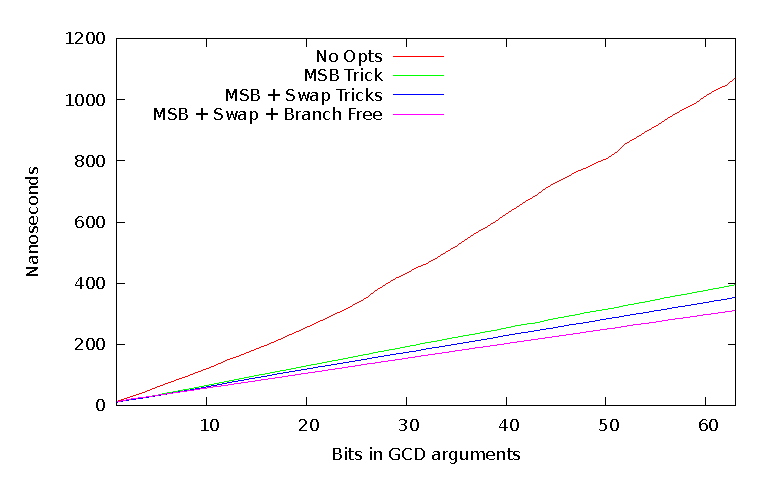
\includegraphics[scale=0.86]{xgcd-binary-optimizations-64}
\end{figure}
\end{frame}


% XGCD QUANTIFIED RESULTS
\begin{frame}
\frametitle{XGCD Improvement}

How much faster than the reference implementations?
\begin{table}
\centering
\begin{tabular}{ | r | l | r | r | r | }
\hline
Bit Range & Algorithm & GMP & Pari & Flint \\
\hline
1 -- 31 & EEA & 3.44 & 1.60 & 1.17 \\
32 -- 63 & Our L2R Binary & 1.94 & 1.29 & 1.16 \\
64 -- 118 & Our L2R Binary & 1.38 & 1.38 & -- \\
119 -- 127 & Lehmer w/ Our 64-bit L2R & 1.12 & 1.13 & -- \\
\hline
\end{tabular}
\end{table}

\bigskip
\smallfont
All times are based on the average.  The measurement of improvement is an average over the bit range.
\end{frame}

% CLASS GROUP IMPROVEMENTS
\begin{frame}
\frametitle{Class Group Improvements}
How much faster than the reference implementations?
\begin{table}
\centering
\begin{tabular}{ | r | r | r | r | }
\hline
Operation & Bit Range & Pari & GMP \\
\hline
Multiplication & 1 -- 59 & 4.27 & 5.66 \\
Squaring & 1 -- 59 & 4.27 & 4.95 \\
Cubing & 1 -- 59 & 5.86 & 4.10 \\
Multiplication & 59 -- 118 & 3.60 & 2.74 \\
Squaring & 59 -- 118 & 4.02 & 2.66 \\
Cubing & 59 -- 118 & 3.82 & 1.83 \\
\hline
\end{tabular}
\end{table}

\bigskip
\smallfont
All times are based on the average.  The measurement of improvement is an average over the bit range.
\end{frame}


%%%%%%%%%%%%%%%%%%%%%%%%%%%%%%%%%%%%%%%%%%%%%%%%%%%%%%%%%%%%%%%%%%%%%%%%%%%%%%%%

% SUPERSPAR
\begin{frame}
\frametitle{Exponentiation Stage of SuperSPAR}
Exponentiate a random form to the product of many odd prime powers.
\[
E = \prod {p_i}^{e_i}
\]
\end{frame}

% 2,3 REPRESENTATIONS
\begin{frame}
\frametitle{2,3 Representations}
\[
N = \sum_{i=0}^k s_i 2^{a_i} 3^{b_i}.
\]
Example:
\begin{itemize}
\item $23814216 = 2^3+2^6+2^{13}+2^{14}+2^{16}+2^{17}+2^{19}+2^{21}+2^{22}+2^{24}$
\item $23814216 = 2^3 3^3 - 2^4 3^5 + 2^5 3^6  + 2^7 3^7 + 2^9 3^8 + 2^{10} 3^9$
\item $23814216 = 2^3 3^3 -2^4 3^6 -2^8 3^5 +2^{15} 3^6$
\item $23814216 = 2^3 3^2 -2^{13} 3^2 +2^{15} 3^6$
\end{itemize}
\end{frame}

\begin{frame}
\frametitle{How to Exponentiate 2,3 Representations?}
First we nest common factors of 2:
\[
2^{15} 3^6 -2^8 3^5 -2^4 3^6 +2^3 3^3 = (((3^6 2^7 - 3^5) 2^4 -3^6) 2^1 +3^3) 2^3
\]
\end{frame}


% HOW TO EXPONENTIATE
\begin{frame}
\frametitle{Exponentiating $g^{2^{15} 3^6 -2^8 3^5 -2^4 3^6 +2^3 3^3}$}
\begin{figure}
\includegraphics[scale=0.70]{yao1}
\end{figure}
\end{frame}
\begin{frame}
\frametitle{Exponentiating $g^{2^{15} 3^6 -2^8 3^5 -2^4 3^6 +2^3 3^3}$}
\begin{figure}
\includegraphics[scale=0.70]{yao2}
\end{figure}
\end{frame}


% L2R BEST APPROXIMATIONS
\begin{frame}
\frametitle{Left-to-Right Best Approximations}
Left-to-Right best approximations is a technique combining the greedy approach of Berth{\'e} and Imbert with the tree based approach of Doche and Habsieger.
\begin{itemize}
\item<2-> Iterate on a set of partial representations $x + \sum s_i2^{a_i}3^{b_i}$.
\item<3-> Keep the best $2^a 3^b$ approximations for each $x$.
\item<4-> Squares and cubes are bound $a \le A$, $b \le B$, and the bounds $A$ and $B$ are iterated.
\end{itemize}
\end{frame}

\begin{frame}
\frametitle{Left-to-Right Best Approximations}
\framesubtitle{Example -- First Iteration on 777}
\begin{figure}
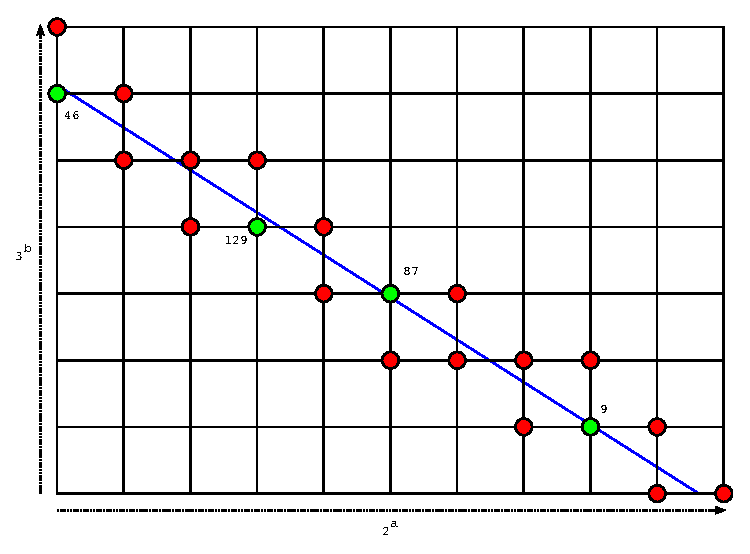
\includegraphics[scale=0.84]{best-approx-777}
\end{figure}
\end{frame}
\begin{frame}
\frametitle{Left-to-Right Best Approximations}
\framesubtitle{Example -- Second Iteration on 9, 48, 87, and 129}
\begin{figure}
\includegraphics[scale=0.84]{best-approx-9-48-87-129}
\end{figure}
\end{frame}
\begin{frame}
\frametitle{Left-to-Right Best Approximations}
\framesubtitle{Example Results}
2,3 Representations for $E=777$:
\begin{align*}
2^8 3^1 + 2^0 3^2 && \textrm{8 squares, 2 cubes, 1 multiplication} \\
2^0 3^6 + 2^4 3^1 && \textrm{4 squares, 6 cubes, 1 multiplication} \\
2^8 3^1 + 2^3 3^0 + 2^0 3^0 && \textrm{8 squares, 1 cube, 2 multiplications} \\
2^3 3^4 + 2^7 3^0 + 2^0 3^0 && \textrm{7 squares, 4 cubes, 2 multiplications}
\end{align*}

\bigskip
$2^8 3^1 + 2^3 3^0 + 2^0 3^0$ possibly preferred since multiplication is cheaper than squaring.
\end{frame}


% EXPONENTIATION IMPROVEMENTS
\begin{frame}
\frametitle{Exponentiation Improvement}
How much faster than the reference implementations?
\begin{table}
\centering
\begin{tabular}{ | l | l | l | l | l | }
\hline
& \multirow{2}{*}{Binary} & \multirow{2}{*}{NAF} & Pruned & Greedy \\
& & & Tree & Left-to-Right \\
\hline
Left-to-Right Best & \multirow{3}{*}{1.40} & \multirow{3}{*}{1.25} & \multicolumn{1}{|r|}{\multirow{3}{*}{1.13}} & \multicolumn{1}{|r|}{\multirow{3}{*}{1.009}} \\
Approximations & & & &\\
(64-bit) & & & &\\

\hline

Left-to-Right Best & \multirow{3}{*}{1.42} & \multirow{3}{*}{1.25} & \multicolumn{1}{|r|}{\multirow{3}{*}{1.18}} & \multicolumn{1}{|r|}{\multirow{3}{*}{1.010}} \\
Approximations & & & &\\
(128-bit) & & & &\\

\hline
\end{tabular}
\end{table}

\bigskip
\smallfont
All times are based on the average.  The measurement of improvement is an average over the bit range.
\end{frame}

% EXPONENTIATION STAGE TEST
\begin{frame}
\frametitle{After Exponentiating}
Exponentiation stage computes:
\[
	q' = q^E.
\]
Then repeatedly square $q'$.
\end{frame}


%%%%%%%%%%%%%%%%%%%%%%%%%%%%%%%%%%%%%%%%%%%%%%%%%%%%%%%%%%%%%%%%%%%%%%

% SEARCH STAGE
\begin{frame}
\frametitle{Search Stage of SuperSPAR}
Use a bounded primorial steps algorithm to find the order of an element (due to Sutherland).
\end{frame}

% PRIMORIALS
\begin{frame}
\frametitle{Primorials}
Primorial:
\[
	P_t = \prod_{p_i \le p_t} p_i.
\]

Coprime to $P_t$:
\[
	\phi(P_t) = \prod_{p_i \le p_t} (p_i - 1).
\]
\end{frame}


% BABY-STEP GIANT-STEP
\begin{frame}
\frametitle{Baby-Step Giant-Step}
Order finding due to Shanks.  Requires $O(\sqrt N)$.

\bigbreak
\begin{algorithmic}[1]
\Require A group element $g$, and a bound on the order $N$.
\State $s \gets \sqrt{N}$
\For{$i = 1, 2, 3, ..., s$}
	\State store $g^i \mapsto i$ in a table
	\If{$g^i = 1_G$} \Return $i$ \EndIf
\EndFor
\For{$j = 1, 2, 3, ..., s$}
	\If{$g^{sj}$ is in the lookup table}
		\State then there exists some $g^i = g^{sj}$
		\State \Return $sj - i$
	\EndIf
\EndFor
\end{algorithmic}
\end{frame}

% ORDER IS ODD
\begin{frame}
\frametitle{What if the Order is Odd?}
Sutherland noticed for odd orders:

\bigbreak
\begin{algorithmic}[1]
\Require A group element $g$, and a bound on the order $N$.
\State $s \gets \sqrt{N/2}$ with $s$ even
\For{$i = 1, 3, 5, ..., s$}
	\State store $g^i \mapsto i$ in a table
	\If{$g^i = 1_G$} \Return $i$ \EndIf
\EndFor
\For{$j = 1, 2, 3, ..., s$}
	\If{$g^{sj}$ is in the lookup table}
		\State then there exists some $g^i = g^{sj}$
		\State \Return $sj - i$
	\EndIf
\EndFor
\end{algorithmic}
\end{frame}

% NO FACTORS OF 2,3 IN ORDER
\begin{frame}
\frametitle{If Both 2 and 3 Do Not Divide the Order?}
Why stop at odd orders?

\bigbreak
\begin{algorithmic}[1]
\Require A group element $g$, and a bound on the order $N$.
\State $s \gets \sqrt{N/3}$ with $s$ a multiple of 6
\For{$i = 1, 5, 7, 11, ..., s$}
	\State store $g^i \mapsto i$ in a table
	\If{$g^i = 1_G$} \Return $i$ \EndIf
\EndFor
\For{$j = 1, 2, 3, ..., s$}
	\If{$g^{sj}$ is in the lookup table}
		\State then there exists some $g^i = g^{sj}$
		\State \Return $sj - i$
	\EndIf
\EndFor
\end{algorithmic}
\end{frame}

% GENERAL CASE
\begin{frame}
\frametitle{General Case}
For all primes up to $p_t$.

\bigbreak
\begin{algorithmic}[1]
\Require A group element $g$, and a bound on the order $N$.
\State $s \gets \sqrt{N/(P_t/\phi(P_t))}$ with $s$ a multiple of $P_t$
\For{$i = 1, ..., s$ with $i$ coprime to $P_t$}
	\State store $g^i \mapsto i$ in a table
	\If{$g^i = 1_G$} \Return $i$ \EndIf
\EndFor
\For{$j = 1, 2, 3, ..., s$}
	\If{$g^{sj}$ is in the lookup table}
		\State then there exists some $g^i = g^{sj}$
		\State \Return $sj - i$
	\EndIf
\EndFor
\end{algorithmic}
\end{frame}

% HOW IS THIS USEFUL?
\begin{frame}
\frametitle{How is This Useful?}

The exponentiation stage computed
\[
	q'' = q^{E\left(2^j\right)}
\]
for
\[
	E = \prod_{i=2}^t {p_i}^{e_i}.
\]
The order of $q''$ is likely coprime to $E$.
\end{frame}

% HOW TO PICK PARAMS
\begin{frame}
\frametitle{How to Pick the Exponent and the Order Bound}
Exponent: Let $p_t \approx N^{1/2r}$ and
\[
	E = \prod_{i=2}^t {p_i}^{e_i}
\]
where $e_i = \log_{p_i} {p_t}^2$.

\bigbreak
Search bound: Maximize $w$ such that $m\phi(P_w) \approx p_t$.

\bigbreak
How to pick $r$ ?
\end{frame}

% Smoothness
\begin{frame}
\frametitle{Smoothness of the Order}
A random number 
\[
m \in [1, N]
\]
is $N^{1/u}$-smooth with probability
\[
u^{-u}.
\]

\bigbreak\bigbreak\bigbreak
\smallfont
${}^*$ See Sutherland for details.
\end{frame}

% MINIMIZE EXPECTED RUNTIME
\begin{frame}
\frametitle{Minimize Expected Running Time}
Assume the order of forms are like random integers.

\begin{itemize}
\item<2-> Group operations per try is $O(N^{1/2r})$
\item<3-> Assume order is random $h \in [1, N^{1/2}]$
\item<4-> Probability of factoring is $r^{-r}$
\item<5-> Expectation is $O(r^r N^{1/2r})$
\item<6-> Minimized for $r = \sqrt{\ln N / \ln \ln N}$
\end{itemize}
\end{frame}


% FAILURE
\begin{frame}
\frametitle{How to Handle Failure?}
\begin{itemize}
\item Try again with a different form.
\item Try again with a different $\Delta = -kN$.
\end{itemize}
\end{frame}

%%%%%%%%%%%%%%%%%%%%%%%%%%%%%%%%%%%%%%%%%%%%%%%%%%%%%%%%%%%%%%%%%%%%%%%

% EVOLUTION OF SUPERSPAR
\begin{frame}
\frametitle{Reference Implementation of SPAR}
\begin{figure}
\includegraphics[scale=0.86]{spar-vanilla}
\end{figure}
\end{frame}
\begin{frame}
\frametitle{Bound the Number of Ideals per Group}
\begin{figure}
\includegraphics[scale=0.86]{spar-bound-attempts}
\end{figure}
\end{frame}
\begin{frame}
\frametitle{Bounded Primorial Steps Search}
\begin{figure}
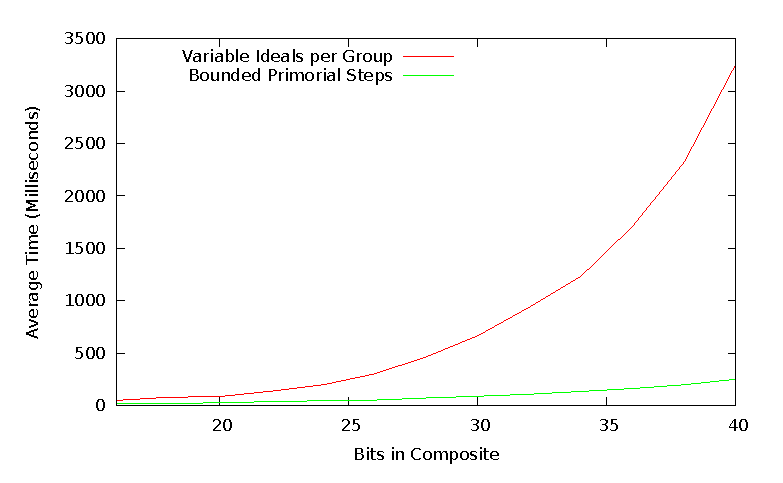
\includegraphics[scale=0.86]{spar-to-sspar}
\end{figure}
\end{frame}
\begin{frame}
\frametitle{Bounded Primorial Steps Search}
\begin{figure}
\includegraphics[scale=0.86]{sspar-theoretical}
\end{figure}
\end{frame}
\begin{frame}
\frametitle{Bound $e_i$ in Exponent $E = \prod {p_i}^{e_i}$}
\begin{figure}
\includegraphics[scale=0.86]{sspar-power-bound}
\end{figure}
\end{frame}
\begin{frame}
\frametitle{Independent Exponent $E$ and Search Bound $mP_w$}
\begin{figure}
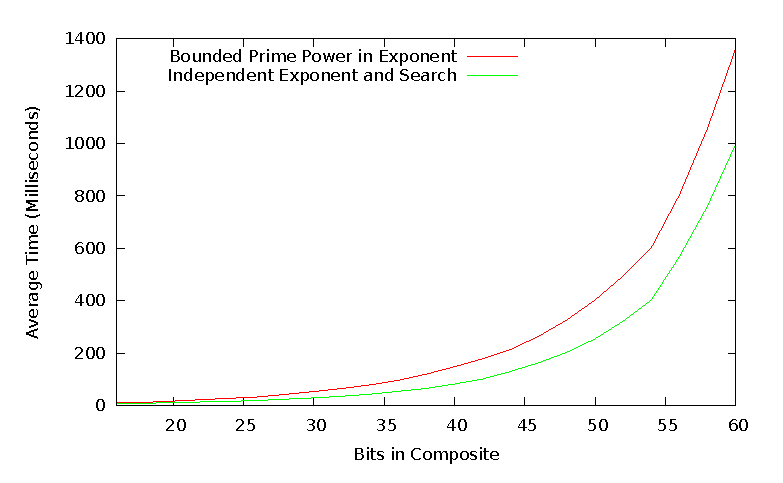
\includegraphics[scale=0.86]{sspar-noreuse}
\end{figure}
\end{frame}
\begin{frame}
\frametitle{Perform a Single Search}
\begin{figure}
\includegraphics[scale=0.86]{sspar-optimized}
\end{figure}
\end{frame}
\begin{frame}
\frametitle{SPAR vs SuperSPAR}
\begin{figure}
\includegraphics[scale=0.86]{spar-vs-sspar}
\end{figure}
\end{frame}


% MEDIAN TIMES
\begin{frame}
\frametitle{Median Integer Factoring Times}
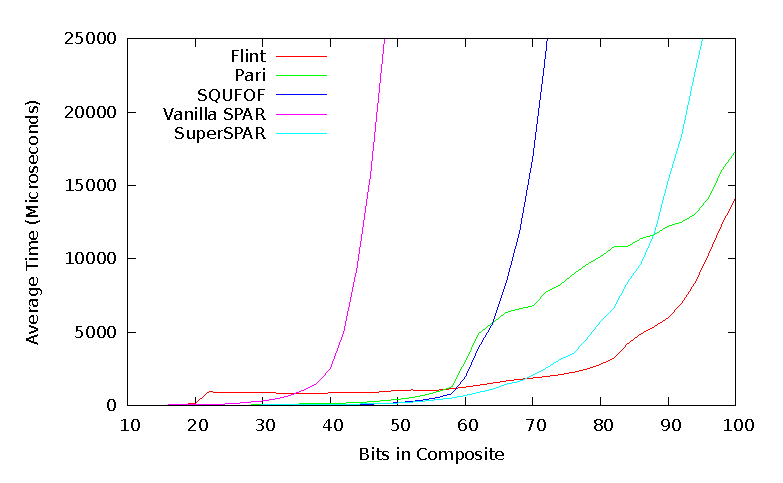
\includegraphics[scale=0.86]{factor-median}
\end{frame}
\begin{frame}
\frametitle{Median Integer Factoring Times (Zoomed Left)}
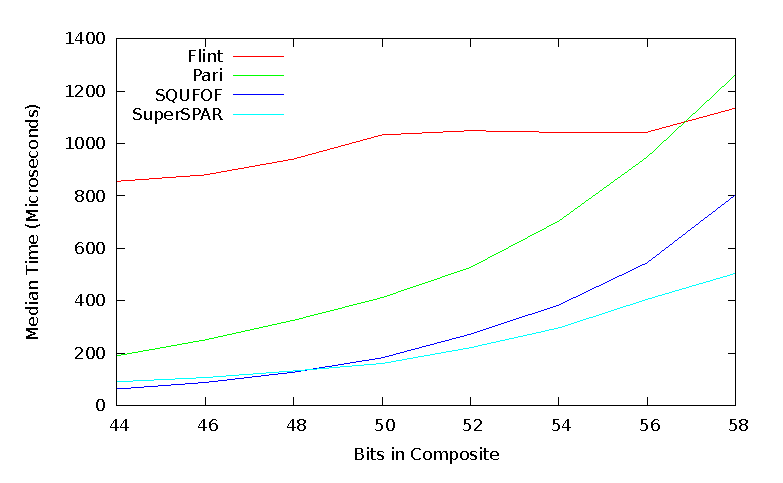
\includegraphics[scale=0.86]{factor-median-zoom-left}
\end{frame}
\begin{frame}
\frametitle{Median Integer Factoring Times (Zoomed Right)}
\includegraphics[scale=0.86]{factor-median-zoom-right}
\end{frame}



%%%%%%%%%%%%%%%%%%%%%%%%%%%%%%%%%%%%%%%%%%%%%%%%%%%%%%%%%%%%%%%%%%%%%%%%%%%%%%%%


% THANK YOU
\begin{frame}
\frametitle{Thank You}
Questions?
\end{frame}

%%%%%%%%%%%%%%%%%%%%%%%%%%%%%%%%%%%%%%%%%%%%%%%%%%%%%%%%%%%%%%%%%%%%%%%%%%%%%%%%

%%%%%%%%%%%%%%%%%%
% END OF DEFENCE %
%%%%%%%%%%%%%%%%%%

\begin{frame}
\end{frame}
\begin{frame}
\end{frame}
\begin{frame}
\end{frame}

% FUTURE WORK
\begin{frame}
\frametitle{Future Work}
Some work that is eagerly awaiting:
\begin{itemize}
\item Special case for quotients $q \le 4$ in XGCD.
\item Real quadratic fields and hyperelliptic curves.
\item Improvements to left-to-right best approximations algorithm.
\end{itemize}
\end{frame}


% SOME USES
\begin{frame}
\frametitle{Some Possible Applications}
These are just a few possible applications. \bigskip

Ideal class group:
\begin{itemize}
\item Class group tabulation for larger discriminants \break (Ramachandran2006).
\end{itemize}

\bigskip
Integer Factoring:
\begin{itemize}
\item Factoring left-overs after sieving in algorithms like the number field sieve using multiple large primes.
\end{itemize}

\end{frame}

% CONTRIBUTIONS TO IDEAL CLASS GROUP ARITHMETIC
\begin{frame}
\frametitle{Contributions}
Contributions to ideal class group arithmetic:
\begin{itemize} %[<+->]
\item Optimized implementations using 64 and 128-bit arithmetic.
\item Optimized XGCD for 32, 64, and 128-bits.
	\begin{itemize}
	\item A simplified left-to-right binary XGCD (and partial XGCD).
	\end{itemize}
\end{itemize}

\bigskip
Contributions to integer factoring:
\begin{itemize}
\item SuperSPAR integer factoring algorithm.
\item Left-to-right best approximations method for computing 2,3 representations of power primorials.
\end{itemize}
\end{frame}

% XGCD
\begin{frame}
\frametitle{Extended Greatest Common Divisor (XGCD)}
Extended greatest common divisor solves
\[
	s = Ua + Vb = \gcd(a, b)
\]
for the largest $s$ dividing both $a$ and $b$.
\end{frame}


% OUR PXGCD
\begin{frame}
\frametitle{Our Left-to-Right Binary PXGCD}
\begin{algorithmic}[1]
\Procedure{Our\_L2R\_PXGCD}{$a, b, T$} \Comment{$a, b, T \in \ZZgez$}
\State $\matrixtt{r_1}{c_1}{r_0}{c_0} \gets \matrixtt{a}{0}{b}{-1}$
\State $z \gets 0, s_1 \gets 1, s_0 \gets 1$
\While {$r_0 \neq 0$ and $r_0 > T$}
	\State $k \gets $ \Call{NumBits}{$r_1$} - \Call{NumBits}{$r_0$}
	\State subtract $2^k$ times the second row from the first
	\If {$r_1 < 0$} $r_1 \gets -r_1, c_1 \gets -c_1, s_1 \gets -s_1$ \EndIf
	\If {$r_1 < r_0$}
		\State swap the rows of the matrix and $s_1$ with $s_0$
		\State $z \gets z + 1$
	\EndIf
\EndWhile
\State \Return $(s_1 \cdot r_1, s_1 \cdot c_1, s_0 \cdot r_0, s_0 \cdot c_0, z)$
\EndProcedure
\end{algorithmic}
\end{frame}



% LEFT-TO-RIGHT BINARY XGCDs
\begin{frame}
\frametitle{Left-to-Right Binary XGCDs}
\framesubtitle{32-bit}
\begin{figure}
\includegraphics[scale=0.86]{xgcds-binary-32}
\end{figure}
\end{frame}
\begin{frame}
\frametitle{Left-to-Right Binary XGCDs}
\framesubtitle{64-bit}
\begin{figure}
\includegraphics[scale=0.86]{xgcds-binary-64}
\end{figure}
\end{frame}
\begin{frame}
\frametitle{Left-to-Right Binary XGCDs}
\framesubtitle{128-bit}
\begin{figure}
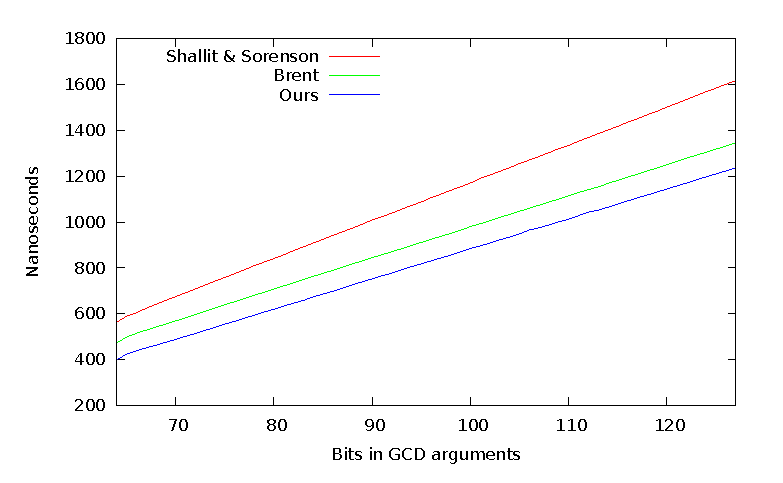
\includegraphics[scale=0.86]{xgcds-binary-128}
\end{figure}
\end{frame}




% SQUARE ROOT APPROXIMATION
\begin{frame}
\frametitle{Approximate Square Root}
Notice that
\begin{equation*}
\begin{array}{rrlrlr}
	& x^{1/2} &=& 2^{(\log_2x)/2} &\approx& 2^{\floor{\floor{\log_2x+1}/2}} \\
	\Rightarrow & x / x^{1/2} &=& x / 2^{(\log_2x)/2} &\approx& x / 2^{\floor{\floor{\log_2x+1}/2}},
\end{array}
\end{equation*}
which is approximated by shifting $x$ right by $\floor{\floor{\log_2x+1}/2}$ bits.
\end{frame}

% SQRT OPTIMIZATION
\begin{frame}
\frametitle{Square Root Approximation}
\framesubtitle{64-bit ideal multiplication}
\begin{figure}
\includegraphics[scale=0.86]{compose-sqrtopt-64}
\end{figure}
\end{frame}

\begin{frame}
\frametitle{Square Root Approximation}
\framesubtitle{128-bit ideal multiplication}
\begin{figure}
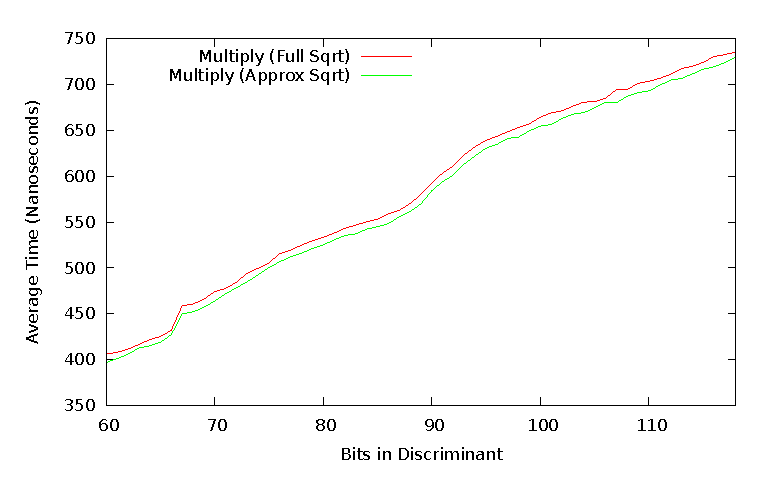
\includegraphics[scale=0.86]{compose-sqrtopt-128}
\end{figure}
\end{frame}

\begin{frame}
\frametitle{Square Root Approximation}
\framesubtitle{64-bit ideal cubing}
\begin{figure}
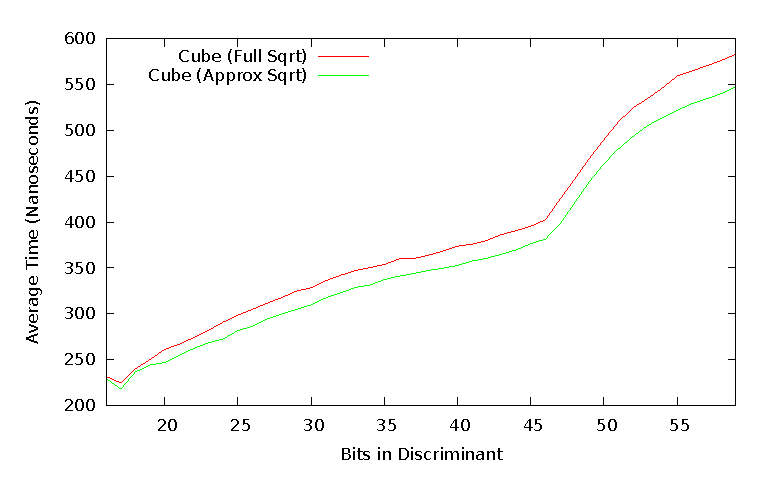
\includegraphics[scale=0.86]{cube-sqrtopt-64}
\end{figure}
\end{frame}

\begin{frame}
\frametitle{Square Root Approximation}
\framesubtitle{128-bit ideal cubing}
\begin{figure}
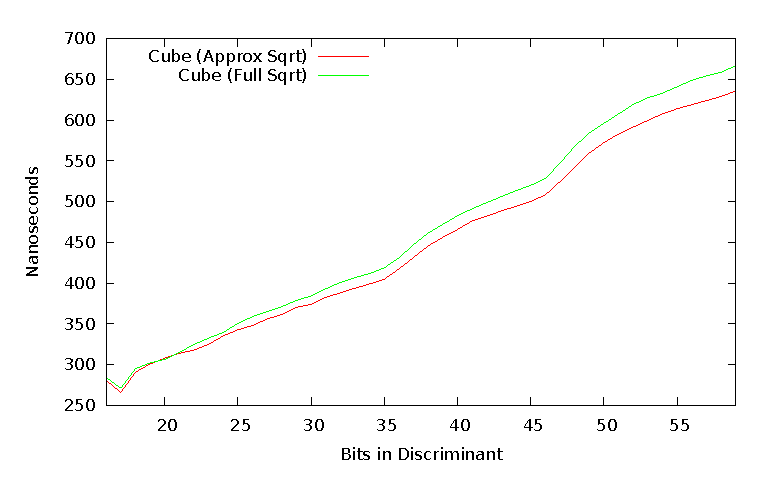
\includegraphics[scale=0.86]{cube-sqrtopt-128}
\end{figure}
\end{frame}


% CUBING -- BIG INTERMEDIATES
\begin{frame}
\frametitle{Large Intermediates During Cubing}
Ideal Cubing (Algorithm 2.4, Page 19).
\begin{align*}
U &= Y'c_1(Y'(b_1 - Y'c_1a_1) - 2) \bmod {a_1}^2 & \textrm{\{line 4\}}\\
U &= -c_1(XY'a_1+Yb_1) \bmod {a_1}^2/s & \textrm{\{line 7\}} \\
M_1 &= \frac{(R_ia_1 + C_iUa_1)}{{a_1}^2} & \textrm{\{line 19\}} \\
M_2 &= \frac{R_i(b_1 + Ua_1) - sC_ic_1}{{a_1}^2} & \textrm{\{line 20\}} \\
\end{align*}
The problem is $a_1 \le \sqrt{|\Delta|/3}$ so ${a_1}^2 \le |\Delta|/3$.
\end{frame}

% GMP WITH 128-BIT CUBING
\begin{frame}
\frametitle{GMP with 128-bit Cubing}
\begin{figure}
\includegraphics[scale=0.86]{smart-cubing-128}
\end{figure}
\end{frame}


% ESTIMATES FOR MANY SIZES
\begin{frame}
\frametitle{Exponentiation Results (16-bit Discriminants)}
\begin{figure}
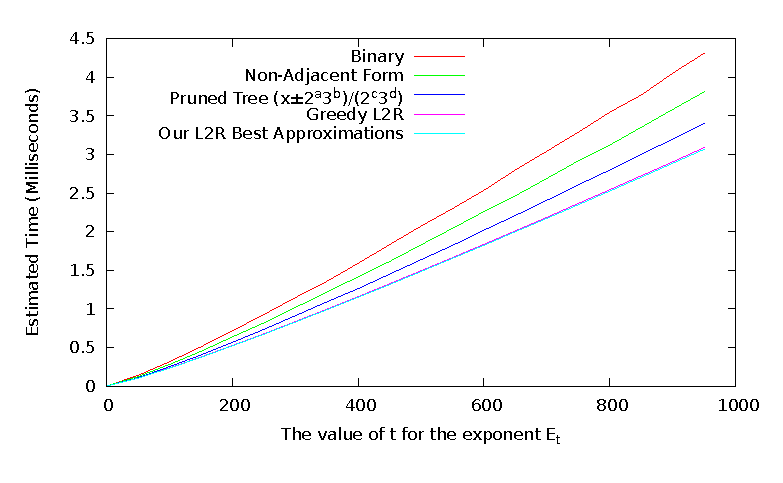
\includegraphics[scale=0.86]{pow-winners-16}
\end{figure}
\end{frame}
\begin{frame}
\frametitle{Exponentiation Results (32-bit Discriminants)}
\begin{figure}
\includegraphics[scale=0.86]{pow-winners-32}
\end{figure}
\end{frame}
\begin{frame}
\frametitle{Exponentiation Results (48-bit Discriminants)}
\begin{figure}
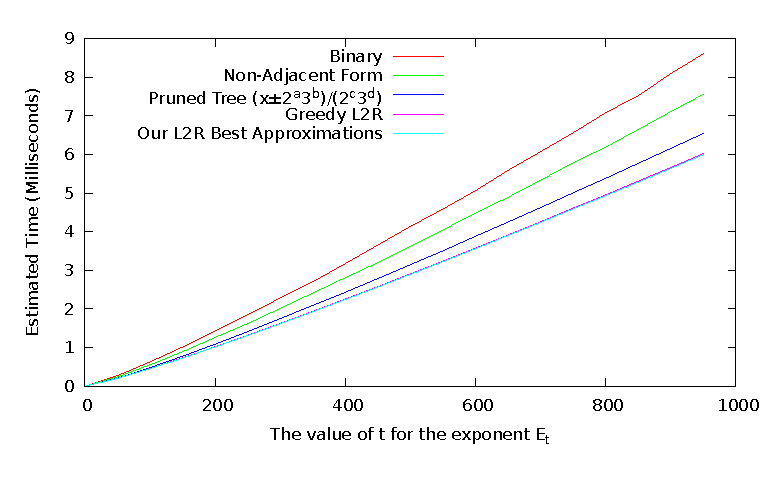
\includegraphics[scale=0.86]{pow-winners-48}
\end{figure}
\end{frame}
\begin{frame}
\frametitle{Exponentiation Results (64-bit Discriminants)}
\begin{figure}
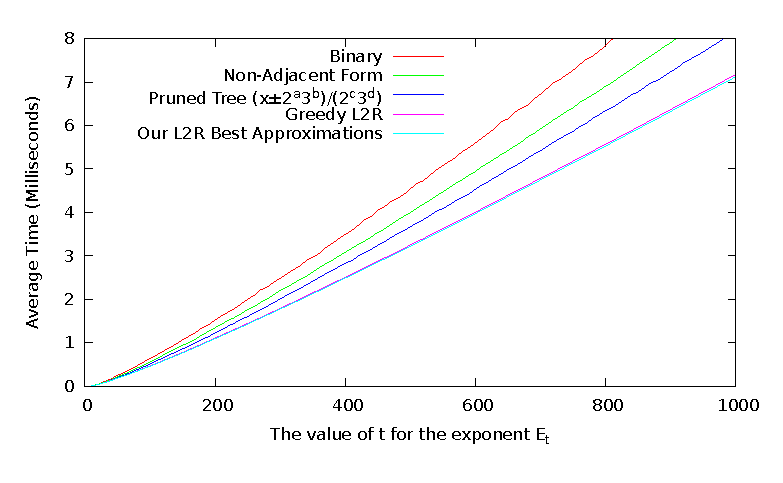
\includegraphics[scale=0.86]{pow-winners-64}
\end{figure}
\end{frame}
\begin{frame}
\frametitle{Exponentiation Results (80-bit Discriminants)}
\begin{figure}
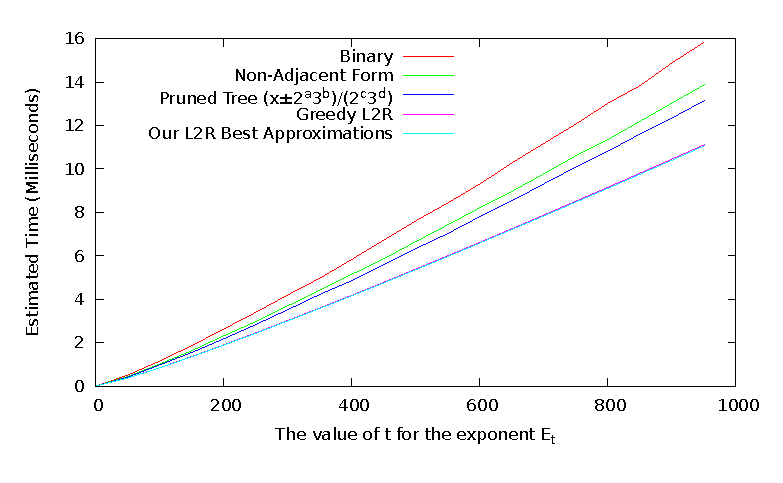
\includegraphics[scale=0.86]{pow-winners-80}
\end{figure}
\end{frame}
\begin{frame}
\frametitle{Exponentiation Results (96-bit Discriminants)}
\begin{figure}
\includegraphics[scale=0.86]{pow-winners-96}
\end{figure}
\end{frame}
\begin{frame}
\frametitle{Exponentiation Results (112-bit Discriminants)}
\begin{figure}
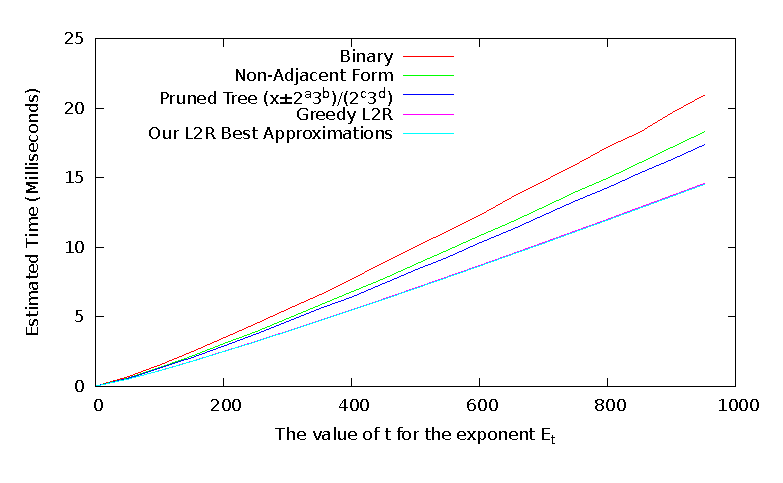
\includegraphics[scale=0.86]{pow-winners-112}
\end{figure}
\end{frame}



% SUPERSPAR
\begin{frame}
\frametitle{SuperSPAR}
SuperSPAR is an integer factoring algorithm based on arithmetic in the ideal class group of imaginary quadratic integers.
\begin{itemize}
\item Extends SPAR using a bounded primorial steps search.
\item Uses improvements to ideal class group arithmetic and 2,3 representations of power primorials.
\item Fastest median time for integers 49-bits to 68-bits of size.
\item Fastest average time for integers 49-bits to 64-bits of size.
\end{itemize}
\bigbreak
\smallfont
Median times do not appear in thesis.
\end{frame}

% THEORETICALLY OPTIMAL PARAMETERS
\begin{frame}
\frametitle{Theoretically Optimal Parameters for Exponentiation Stage}
\begin{table}
\centering
\begin{tabular}{| r | r | r | r | r |}
\hline
$\log_2 N$ & $r = \sqrt{\ln N / \ln \ln N}$ & $\floor{N^{1/2r}}$ & $p_t$ & $t$ \\
\hline
16 & 2.14693 & 13 & 13 & 6 \\
32 & 2.67523 & 63 & 61 & 18 \\
48 & 3.08112 & 221 & 211 & 47 \\
64 & 3.42016 & 655 & 653 & 119 \\
80 & 3.71609 & 1738 & 1733 & 270 \\
96 & 3.98139 & 4258 & 4253 & 583 \\
112 & 4.22355 & 9802 & 9791 & 1208 \\
128 & 4.44745 & 21473 & 21467 & 2407 \\
\hline
\end{tabular}
\end{table}
\end{frame}

% THEORETICALLY OPTIMAL SEARCH BOUNDS
\begin{frame}
\frametitle{Theoretically Optimal Search Bounds}
\begin{table}
\centering
\begin{tabular}{| r | r | r | r | r | r |}
\hline
$\log_2 N$ & $\floor{N^{1/2r}}$ & $2m\phi(P_w)$ & $m^2\phi(P_w)P_w$ & $m$ & $w$ \\
\hline
16 & 13 & 16 & 480 & 1 & 3 \\
32 & 63 & 64 & 7680 & 4 & 3 \\
48 & 221 & 224 & 94080 & 14 & 3 \\
64 & 655 & 656 & 806880 & 41 & 3 \\
80 & 1738 & 1824 & 7277760 & 19 & 4 \\
96 & 4258 & 4320 & 40824000 & 45 & 4 \\
112 & 9802 & 10080 & 222264000 & 105 & 4 \\
128 & 21473 & 22080 & 1173110400 & 23 & 5 \\
\hline
\end{tabular}
\end{table}
\end{frame}


% FACTORIZATION OF THE ORDER, E.G. 1
\begin{frame}
\frametitle{Factorization of the Order}
\framesubtitle{Example \#1}

$N = 9223375433619660527, k = 1, \Delta = -kN$
\begin{itemize}
\item $\ord(\idealclass{p_{19}}) = 2^2 \cdot 13 \cdot 2770667$
\item $\ord(\idealclass{p_{37}}) = 2^3 \cdot 3 \cdot 13 \cdot 2770667$
\item $\ord(\idealclass{p_{43}}) = 2^4 \cdot 3 \cdot 13 \cdot 2770667$
\item $\ord(\idealclass{p_{47}}) = 2^3 \cdot 3 \cdot 13 \cdot 2770667$
\item $\ord(\idealclass{p_{59}}) = 2^4 \cdot 3 \cdot 13 \cdot 2770667$
\end{itemize}

where $\ideal p_p = [p, (b + \sqrt\Delta)/2]$.

\bigskip
Each prime ideal split $N$.
\end{frame}

% FACTORIZATION OF THE ORDER, E.G. 2
\begin{frame}
\frametitle{Factorization of the Order}
\framesubtitle{Example \#2}

$N = 18278283564428467183, k = 3, \Delta = -4kN$
\begin{itemize}
\item $\ord(\idealclass{p_{11}}) = 2 \cdot 3 \cdot 59 \cdot 157 \cdot 1451$
\item $\ord(\idealclass{p_{17}}) = 2 \cdot 5^2 \cdot 59 \cdot 157 \cdot 1451$
\item $\ord(\idealclass{p_{23}}) = 2 \cdot 3 \cdot 5^2 \cdot 59 \cdot 157 \cdot 1451$
\item $\ord(\idealclass{p_{29}}) = 2 \cdot 3 \cdot 59 \cdot 157 \cdot 1451$
\item $\ord(\idealclass{p_{31}}) = 2 \cdot 5 \cdot 59 \cdot 157 \cdot 1451$
\end{itemize}

where $\ideal p_p = [p, (b + \sqrt\Delta)/2]$.

\bigskip
Only $\idealclass{p_{23}}$ and $\idealclass{p_{29}}$ split $N$.

\end{frame}

% REUSING THE ORDER
\begin{frame}
\frametitle{Reusing the Order}
Once the order of an ideal class is known, we skip the search phase.
\begin{itemize}
\item The exponentiation stage removed all small primes $\Rightarrow$ search stage not necessary.
\item The exponentiation stage did not remove all small primes $\Rightarrow$ stepping coprime will never find the order.
\end{itemize}
For $N \le 2^{80}$, this is expected to work better than 97.7\% of the time.
\end{frame}

% 3D SUPERSPAR SEARCH SPACE
\begin{frame}
\frametitle{SuperSPAR Search Space}
\framesubtitle{48-bit semiprimes}
\begin{figure}
\includegraphics[scale=0.47]{bits-48-3d.png}
\end{figure}
\end{frame}
\begin{frame}
\frametitle{SuperSPAR Search Space}
\framesubtitle{56-bit semiprimes}
\begin{figure}
\includegraphics[scale=0.47]{bits-56-3d.png}
\end{figure}
\end{frame}
\begin{frame}
\frametitle{SuperSPAR Search Space}
\framesubtitle{64-bit semiprimes}
\begin{figure}
\includegraphics[scale=0.47]{bits-64-3d.png}
\end{figure}
\end{frame}
\begin{frame}
\frametitle{SuperSPAR Search Space}
\framesubtitle{72-bit semiprimes}
\begin{figure}
\includegraphics[scale=0.47]{bits-72-3d.png}
\end{figure}
\end{frame}
\begin{frame}
\frametitle{SuperSPAR Search Space}
\framesubtitle{80-bit semiprimes}
\begin{figure}
\includegraphics[scale=0.47]{bits-80-3d.png}
\end{figure}
\end{frame}

\begin{frame}
\frametitle{SuperSPAR Prime Ideals}
\framesubtitle{Sequential vs Random}
\begin{figure}
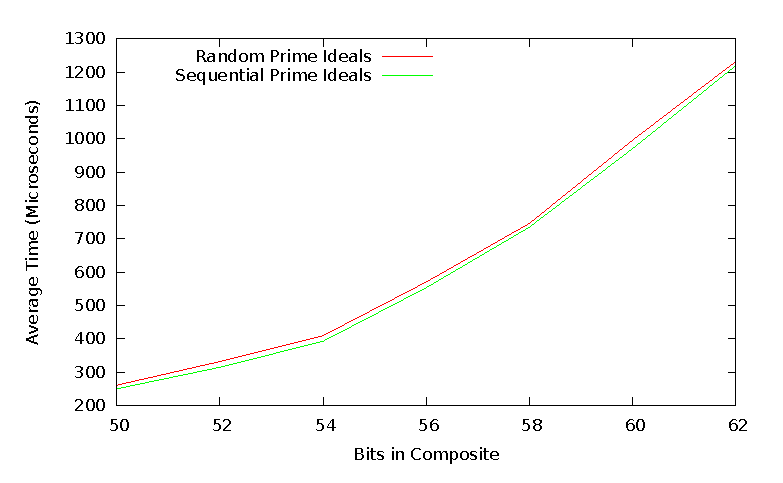
\includegraphics[scale=0.86]{sspar-random-vs-sequential}
\end{figure}
\end{frame}


\begin{frame}
\frametitle{SPAR -- Expanding the 2-Sylow Group}
\begin{table}
\centering
\begin{tabular}{| r | r | r |}
	\hline
	Bits & With 2-Sylow Group & Without 2-Sylow Group \\
	\hline
	16 &   48.05208 &   48.02160 \\
	20 &   84.20318 &   84.09526 \\
	24 &  197.02479 &  196.84587 \\
	28 &  463.70674 &  463.60538 \\
	32 &  937.57875 &  935.81785 \\
	36 & 1709.55629 & 1706.32960 \\
	40 & 3255.31447 & 3248.67998 \\
	\hline
\end{tabular}
\caption{Average time in microseconds to factor using SPAR when the number of ideals per class group is bound by the size of the integer to factor.}
\end{table}
\end{frame}

% BOX AND WHISKER PLOTS
\begin{frame}
\frametitle{Flint}
\begin{figure}
\includegraphics[scale=0.86]{factor-flint-whisker}
\end{figure}
\end{frame}
\begin{frame}
\frametitle{Pari}
\begin{figure}
\includegraphics[scale=0.86]{factor-pari-whisker}
\end{figure}
\end{frame}
\begin{frame}
\frametitle{SQUFOF (Optimized from Pari)}
\begin{figure}
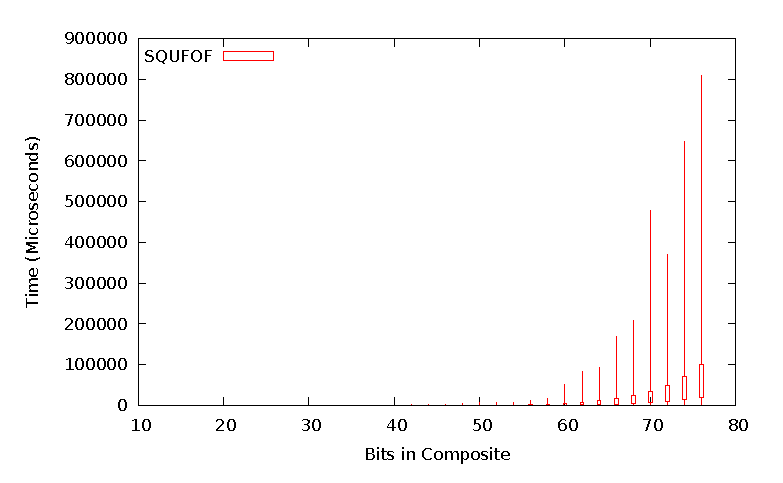
\includegraphics[scale=0.86]{factor-squfof-whisker}
\end{figure}
\end{frame}
\begin{frame}
\frametitle{Vanilla SPAR}
\begin{figure}
\includegraphics[scale=0.86]{factor-spar-whisker}
\end{figure}
\end{frame}
\begin{frame}
\frametitle{SuperSPAR}
\begin{figure}
\includegraphics[scale=0.86]{factor-sspar-whisker}
\end{figure}
\end{frame}

% AVERAGE TIMES
\begin{frame}
\frametitle{Average Integer Factoring Times}
\includegraphics[scale=0.86]{factor-average}
\end{frame}
\begin{frame}
\frametitle{Average Integer Factoring Times (Zoomed Left)}
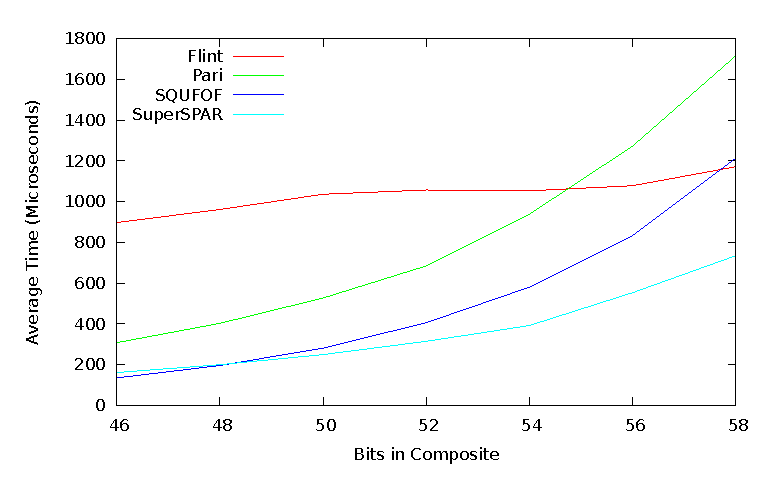
\includegraphics[scale=0.86]{factor-average-zoom-left}
\end{frame}
\begin{frame}
\frametitle{Average Integer Factoring Times (Zoomed Right)}
\includegraphics[scale=0.86]{factor-average-zoom-right}
\end{frame}

% SIMPLE CONTINUED FRACTION EXPANSION
\begin{frame}
\frametitle{Simple Continued Fraction Expansion of $K / L$}
Recurrences:
\begin{align*}
R_i &= R_{i-2} - q_i R_{i-1} \\
C_i &= C_{i-2} - q_i C_{i-1} \\
A_i &= A_{i-2} + q_i A_{i-1} \\
B_i &= B_{i-2} + q_i B_{i-1}
\end{align*}

Invariants:
\begin{align*}
C_i &= (-1)^{i+1} B_i \\
L &= R_iB_{i-1} + B_iR_{i-1} \\
(-1)^{i-1} &= A_iB_{i-1} - B_iA_{i-1} \\
(-1)^{i+1} R_i &= LA_i - KB_i \\
\end{align*}
\end{frame}

\end{document}

